\documentclass[compress, aspectratio=169]{beamer}

%presentation layout

\mode<presentation>
{
  \usetheme{Berlin}
  % \usecolortheme{dove}
  \setbeamercolor{structure}{bg=white,fg=black}
  \setbeamercolor{normal text}{bg=white,fg=black}
  \setbeamercolor{titlepage}{bg=white,fg=black}
  \setbeamercolor{titlelike}{bg=white,fg=black}
  \setbeamercolor{palette primary}{bg=white}
  \setbeamercolor{palette secondary}{bg=gray, fg=white}
  \setbeamercolor{palette tertiary}{bg=gray, fg=white}
  \setbeamercolor{palette quarternary}{bg=white}
  \setbeamercovered{transparent}
  \useinnertheme{rectangles}
  %\usefonttheme{serif}
}

\setbeamertemplate{navigation symbols}{}

%loading packages
\usepackage[ngerman]{babel}
\usepackage[T1]{fontenc}
\usepackage[utf8]{inputenc}
\usepackage{graphicx}
\usepackage{amsmath}
\usepackage{framed}

% vorgeplaenkel
\title[StAPf-Bericht]{StAPF-Bericht}

\author{Ständiger Ausschuss aller Physikfachschaften}

\institute[Zusammenkunft aller Physikfachschaften]

\date{31. Oktober 2019}

\subject{Bericht des StAPF}

\begin{document}

\begin{frame}[plain]{}
  \titlepage
\end{frame}

\section{Zusammensetzung}

\begin{frame}{Aktuelle Zusammensetzung}
  \begin{itemize}
  \item \emph{Andreas Drotloff (Uni Würzburg)}
  \item \emph{Christoph Blattgerste (Uni Heidelberg)}
  \item \emph{Leon Nutzinger (FU Berlin)}
  \item Chantal Beck (Uni Würzburg)
  \item Victoria Schemenz (Alumna)
  \end{itemize}
\end{frame}

\section{Was bisher geschah...}

\begin{frame}{Was bisher geschah...}
  \begin{itemize}
  \item Resolutionen verschickt und veröffentlicht
    \begin{itemize}
        \item Resolution zu den Akkreditierungsrichtlinien
        \item Resolution zu universitärer Selbstverwaltung
        \item Resolution zur Unterstützung des BAföG-Bündnisses
        \item Resolution zur Verurteilung von Onlineplattformen zur Denunziation von Lehrenden
        \item Resolution zu Verfassten Studierenschaften      
        \item Resolution zur Zivilklausel NRW
        \item Positionspapier zu Fortgeschrittenenpraktika
    \end{itemize}
  \end{itemize}
\end{frame}

\begin{frame}
  \begin{itemize}
    \item ZaPF-Bericht verschickt und veröffentlicht
    \item 7 Sitzungen seit der ZaPF in Bonn
    \item Klausurtagung vom 26.-28.07.19 in Freiburg zur Nachbereitung von Bonn
    \item Klausurtagung vom 13.-15.09.19 in Erlangen zur Vorbereitung von Freiburg
    \end{itemize}
    \vspace{5mm}
    \begin{center}
      \Large DANKE an alle, die uns dabei unterstützt haben!
    \end{center}
\end{frame}

%\section{Rückmeldungen}

%\begin{frame}{BMBF}
 %   \item Es gab eine Anfrage und zwei Nachfragen an das BMBF
  %   \item Antwort: Nicht genügend Mittel in Förderrunde 2017/2018
   %  \item Prinzipiell steht einer Förderung der nächsten ZaPFen nichts entgegen
 % \end{itemize}
%\end{frame}


\section{Akkreditierung}

%unvollständig
% Edit: pjaeger. Fixed typo
\begin{frame}{Akkerditierungspool}
    \begin{itemize}
        \item Der studentische Akkreditierungspool
        \begin{itemize}
        	\item sorgt für die Einflussnahme von Studierenden in Akkreditierungsverfahren
        	\item entsendet Studierendenvertreter in den Akkreditierungsrat und in Agentur- und (extern besetzte) Hochschulgremien
        	\item vertritt studentische Interessen gegenueber Agenturen und anderen Stakeholdern
\end{itemize}         
        \item Studierende werden vorher in Seminaren geschult. \\
        {\scriptsize\color{blue} N"achste Termine: 8.-10.11. Bamberg, 15.-17.11. K"oln}
        % Edit: pjaeger. Ort PVT und Dollarzeichen bei rightarrow
        \item Nächstes Poolvernetzungstreffen in Dresden {\color{blue} (29. November bis 01. Dezember)}
        \vspace{0.5cm}
        \item[$\rightarrow$] Bei Interesse: Besucht den Akkreditierungs-Workshop f"ur Einsteiger bzw. die Akkreditierungs-AKs
    \end{itemize}
\end{frame}

\begin{frame}{Akkreditierunspool}{Aktuelles}
	\begin{itemize}
		\item Akkreditierung im neuen System: Behandlung der ersten Verfahren im Akkreditierungsrat
		\item Schaffung einer Beschwerdekommission beim AR, an die sich auch Studierende direkt wenden k"onnen
		\item "Uberarbeitetes Schulungsseminar (neues Recht, Planspiel, Kommunikationstechniken)
		\item Neuauflage der fachspezifischen Hinweise zur Physik bei ASIIN
		\item Fachsiegel Physik
	\end{itemize}
\end{frame}

\begin{frame}{Akkreditierunspool}{"Anderung der ASIIN-FEH}
	\begin{itemize}
		\item Wesentliche Vorarbeit der Akkreditierungs-AKs (Danke! an Daniela und Lars)
		\item Sollen auf der n"achsten Sitzung am 19.11. beschlossen werden
	\end{itemize}
	\pause
	\begin{block}{Wesentliche "Anderungen}
	\begin{itemize}
		\scriptsize
		\item Beschreibung des Curriculums: \textit{\glqq Das Studium vermittelt alle zum erfolgreichen Studienabschluss notwendigen Fähigkeiten z.B. im Rahmen von geeignet gestalteten Wahlbereichen.\grqq}
		%TODO Reference to ESG
		\item Bef"ahigung zum gesellschaftlichen Engagement (MRVO \S 11, diverse Bologna-Kommuniqu\'es), Wissenschaftskommunikation, sowie wissenschaftstheoretische und ethische Gesichtspunkte als Studiengangsziele
		\item "Uberfachliche Qualifikationen enthalten jetzt Pr"asentationstechniken und Programmierkenntnisse 
	\end{itemize}		
	\end{block}
\end{frame}

\section{MeTaFa}

 \begin{frame}{MeTaFa}
  \begin{itemize}
    \item Treffen in Erlangen (13. bis 15. September 2019)
    \item Die ZaPF war vertreten durch Merten Dahlkemper und Peter Steinmüller
    \item Darum gings:
    \begin{itemize}
        \item Verabschiedung von gemeinsamen Resolutionen
        \item Studienführer 4all
        \item Umsetzung der DSGVO
    \end{itemize}
    \item Nächstes Treffen: In Dortmund (???)
   \end{itemize}
 \end{frame}

\section{Kommende ZaPFen}
\begin{frame}{Kommende ZaPFen}
  \begin{itemize}
    \item Sommersemester 2020 in Rostock und Greifswald
    % \vspace{05cm}
    \item Wintersemester 2020 in \textcolor{blue}{\textit{Hier könnte deine Uni stehen}}
    \item Sommersemester 2021 in \textcolor{blue}{\textit{Hier könnte deine Uni stehen}}
    \end{itemize}
\end{frame}

\begin{frame}[plain]
  \begin{center}
    \Huge Habt ihr Fragen an uns?
    \end{center}
\end{frame}

\section{KommGrem}

 \begin{frame}{KommGrem}
  
  ZaPF:
  \begin{itemize}
   \item Jacob Brunner (Uni Augsburg)
   \item \textit{Sebastian Blänsdorf (Uni Heidelberg)}
  \end{itemize}
  
  jDPG:
  \begin{itemize}
   \item Anastasia Boushmelev (Uni Siegen)
   \item Merten Dahlkemper (Uni Göttingen)
  \end{itemize}

 \end{frame}
 

 \begin{frame}{Was bisher geschah...}
  \begin{itemize}
   \item jDPG Mitgliederversammlung (Niklas, Anas \& Merten)
   \item CHE Fachbeirat (Fredrica \& Thomi)
   \item Vorbereitung BaMa-Umfrage
   \item Konferenz der Fachbereiche Physik
   \begin{itemize}
    \item KFP in Berlin (6.11.2017 - Fredrica \& Merten)
    \item KFP in Bad Honnef (22./23.5.2018 - Sonja \& Merten)
   \end{itemize}
  \end{itemize}
 \end{frame}
 
 
 \begin{frame}{KFP Dauerbrenner-Themen}
  \begin{itemize}
   \item Berichte DPG Vorstand, Math.-Nat. Fakultätentag, ... 
   \item Bereinigung der Studierendenstatistik von 'Parkstudierenden'
   \item Ars Legendi Fakultätenpreis
   \item CHE-Ranking
   \item Akkreditierung
   \item Studienatlas
  \end{itemize}
 \end{frame}
 
 
 \begin{frame}{KFP aktuelle Themen}
 
  Berlin:
  \begin{itemize}
   \item Mathematische Lernvoraussetzungen für MINT-Studiengänge
   \item Physik für Medizinerinnen und Mediziner
   \item Promotionsstudie
  \end{itemize}
  
  \bigskip
  
  Bad Honnef:
  \begin{itemize}
   \item Vorstellung neuer DPG Präsident (Dieter Meschede)
   \item Bericht DFG 
   \item Bericht Akkreditierungsrat 
   \item Open Science Policy Platform 
  \end{itemize}
 \end{frame}

%\section{ZaPF e.V.}

\thispagestyle{empty}
\begin{frame}
  \begin{center}
    \Large{ ZaPF e.V. Bericht }\\
    \vspace{1cm}
    \large Zusammenkunft aller Physik Fachschaften e.V.\footnote{nicht mit Z.A.P.F.e.V. zu verwechseln ;-)}\\
    \vspace{0.5cm}
    \normalsize 31. Oktober 2019
  \end{center}
\end{frame}

\thispagestyle{empty}
\begin{frame}{Was ist der ZaPF e.V.?}
für uns sieht das etwa so aus: \\
  \begin{center}
    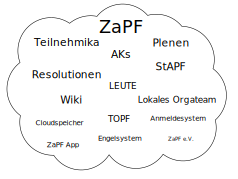
\includegraphics[width=0.6\textwidth]{uns}
  \end{center}
\end{frame}

\thispagestyle{empty}
\begin{frame}{Was ist der ZaPF e.V.?}
von außen sieht das etwa so aus: \\
  \begin{center}
    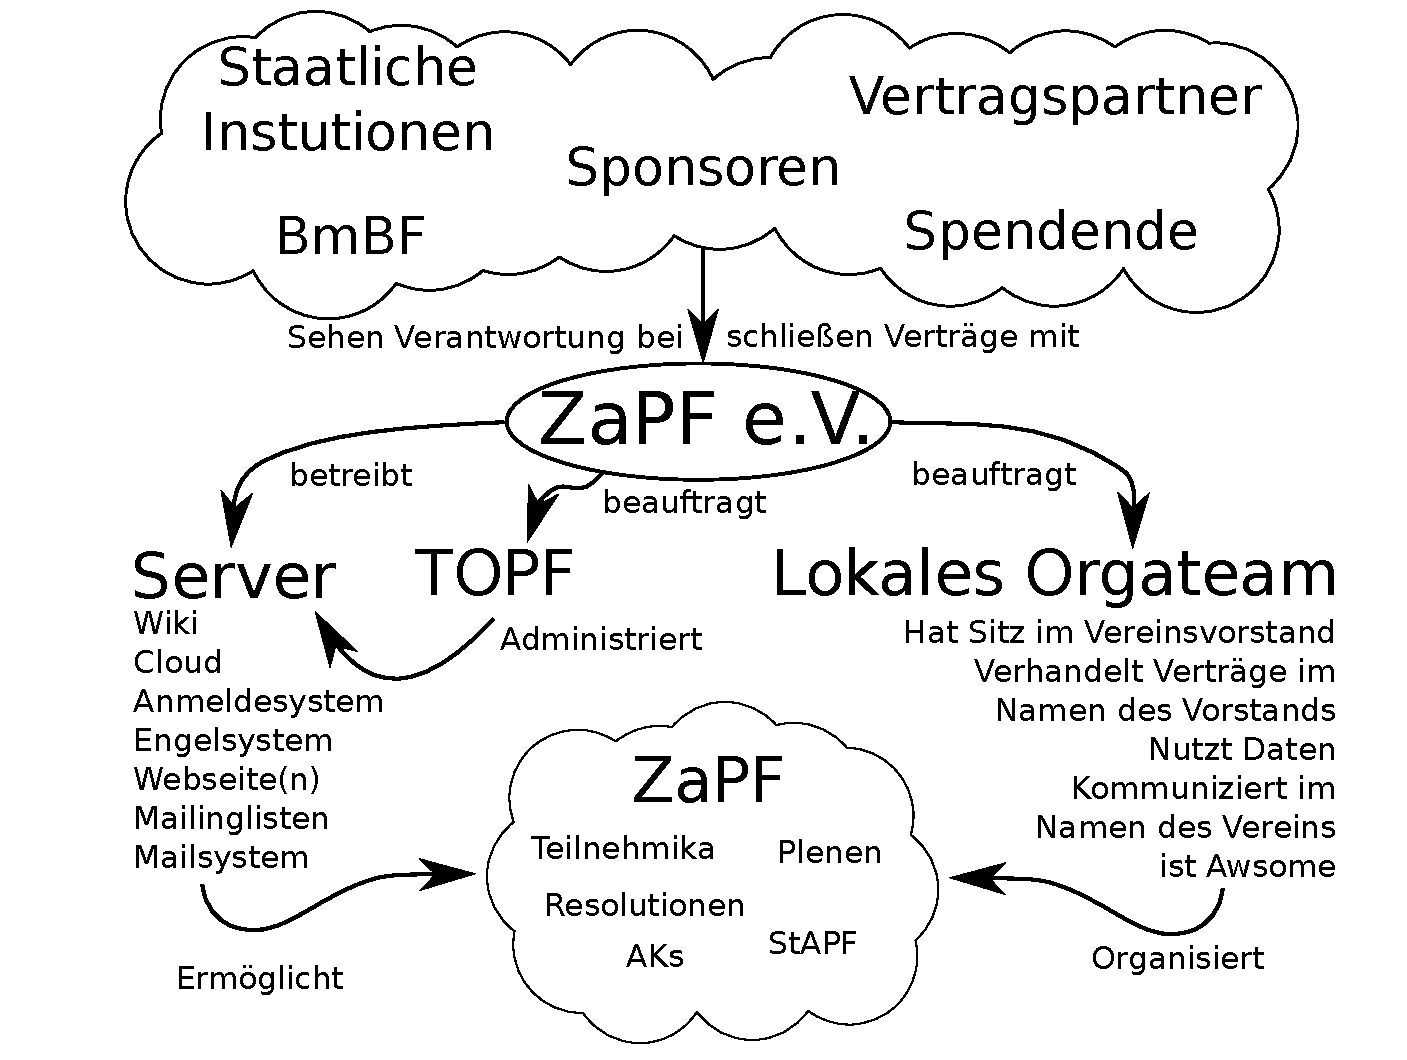
\includegraphics[width=0.56\textwidth]{aussen}
  \end{center}
\end{frame}

\pagestyle{empty}
\begin{frame}{Was tut der ZaPF e.V.?}
\begin{block}{Aufgaben des e.V.:}
\begin{itemize}
\item Strukturelle Unterstützung der ZaPF
\item Infrastruktur
\item Finanzielle Absicherung
\item Rechtliche Absicherung
\item Förderung von Finanzschwachen Fachschaften und mehr
\end{itemize}
\end{block}
\pause
\begin{block}{Aktuelle Aufgaben}
Dokumentation der Prozesse um diese Absicherung besser leisten zu können
\end{block}
\end{frame}

\thispagestyle{empty}
\begin{frame}{Prozesse formalisieren:}
  \begin{center}
    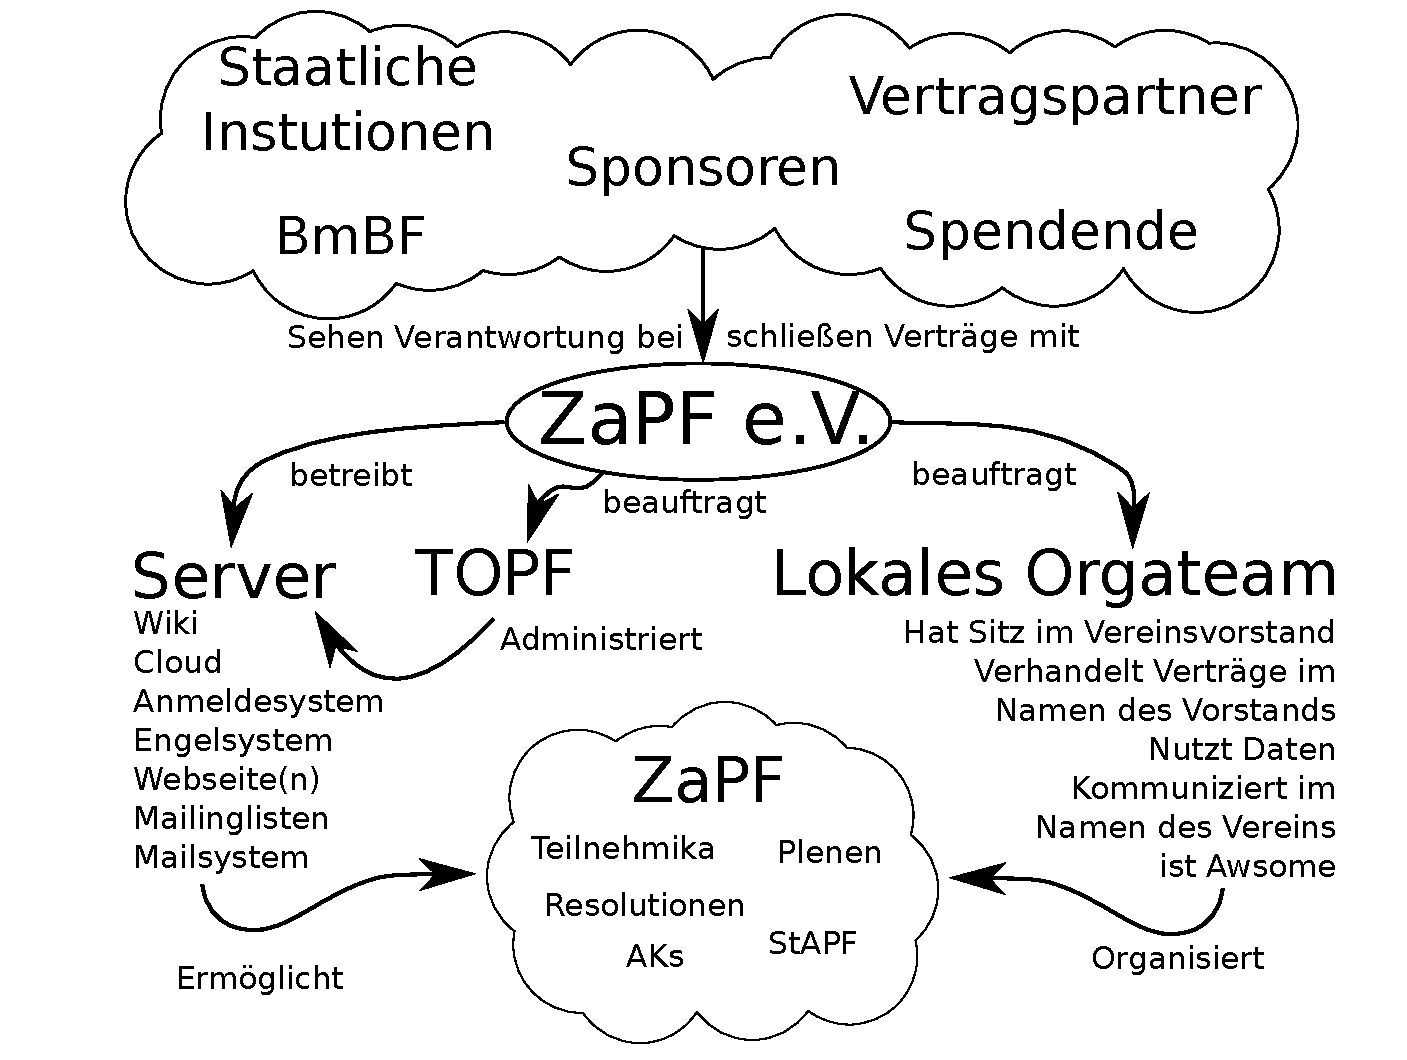
\includegraphics[width=0.56\textwidth]{aussen}
  \end{center}
    für rechtliche Absicherung \& vielleicht sogar hilfreich
\end{frame}


\thispagestyle{empty}
\begin{frame}{Wer tut da was im ZaPF e.V.?}
    \begin{itemize}
        \item[] aktueller Vorstand:
        \begin{itemize}
             \item Peter Steinmüller (KIT) (1. Vorsitz)
             \item Daniela Kern-Michler (Uni Frankfurt) (2. Vorsitz)
             \item Jens Borgemeister (Uni Siegen) (Finanzen)
             \item Marcus Mikorski (KIT) (2. Finanzen)
             \item Tobias Löffler (HHU) (Mitglieder)
             \item Fabian Freyer (TUB) (IT Vorstand)
             \item Lisa Dietrich (Uni Erlangen-Nürnberg)  (Finanzschwache Fachschaften)
             \item Jan Gräfje (Uni Heidelberg)
             \item Andreas Drotloff (Uni Würzburg)
             \item Marcel Nitsch (Uni Bonn)
             \item Timo Rachel (Uni Freiburg)
             \item Richard Altenkirch (Uni Rostock)
        \end{itemize}
    \end{itemize}
\end{frame}

\thispagestyle{empty}
\begin{frame}{Was kann man tun im ZaPF e.V.?}
  \begin{block}{Mitglied werden}
    Mitgliederversammlung:
    \begin{itemize}
      \item Tätigkeitsberichte
      \item Strukturänderungen
      \item ...
    \end{itemize}
  \end{block}
\pause
  \begin{block}{Fördermitglied werden}
  Fachschaften unterstützen den e.V. mit Mitgliedsbeiträgen
  \end{block}
\end{frame}

\thispagestyle{empty}
\begin{frame}
  \begin{center}
    \Large{ TOPF Bericht }\\
    \vspace{1cm}
    \large Technisches Organisationsgremium der Physikfachschaften\\
    \vspace{0.5cm}
    \normalsize 31. Oktober 2019
  \end{center}
\end{frame}

\thispagestyle{empty}
\begin{frame}{Was ist der TOPF?}
  \begin{itemize}
    \item 2 DECkEL\footnote{Dokumentations-, Einrichtungs- und Clusterfuckkoordinierende für EDV-Lösungen} 
    \begin{itemize}
      \item Sean Bonkwoski (Bonn)
      \item Timo Prinz (Berlin, TU)
    \end{itemize}
    \item Viele HENkeL\footnote{Helfende mit EDV- und Netzwerkkompetenzen für ergebnisorentierte Lösungen}\footnote{Können gerne mehr werden ;-)}
    \item Server
    \item ... und ganz viele Dienste
  \end{itemize}
\end{frame}

\thispagestyle{empty}
\begin{frame}{... und ganz viele Dienste}
  \begin{itemize}
    \item ZaPF-Wiki (zapf.wiki)
    \item Studienführer (studienführer-physik.de)
    \item ZaPF-App (app.zapf.in)
    \item Auth-System, \glqq{}ZaPF-Account\grqq{} (auth.zapf.in)
    \item Anmeldesystem (anmeldung.zapf.in)
    \item Webseite für ZaPF e.V. (zapfev.de)
    \item WOLKe\footnote{Wissens-Online-Lager für Kompetenzerhaltung} (Nur für Gremienarbeit)
    \item ... und viele mehr!
  \end{itemize}
\end{frame}

\pagestyle{empty}
\begin{frame}{Was tut der TOPF?}
\begin{block}{Aufgaben der DECkEL:}
\begin{itemize}
\item Vorhandene Dienste am laufen und aktuell halten
\item Gremika Rechte geben und entziehen
\item Dienste für Orgas der nächsten ZaPFen bereitstellen
\item HENkeL koordiniern
\end{itemize}
\end{block}
\pause
\begin{block}{Aufgaben der HENkeL}
  \begin{itemize}
    \item Entwicklung und Einrichtung neuer Dienste
    \item Generell Hilfe und Entlastung der DECkEL
  \end{itemize}
\end{block}
\end{frame}

\pagestyle{empty}
\begin{frame}{Was hat der TOPF seit Bonn getan?}
  \begin{itemize}
    \item WOLKe\footnote{Wissens-Online-Lager für Kompetenzerhaltung} eingerichtet (Nur für Gremienarbeit)
    \item ZapF-Wiki-Anmeldung jetzt über ZaPF-Account
    \item Datenschutz-Überarbeitung mit ZaPF-e.V.-Vorstand
    \item Dinge für ZaPF in Freiburg (Anmeldung, App, ...)
  \end{itemize}
\end{frame}

\pagestyle{empty}
\begin{frame}{Was hat der TOPF noch zu tun?}
  Arbeit geht uns nie aus.
  \begin{itemize}
    \item Alten Server abschalten (fast fertig!)
    \item Backups!
    \item Datenschutz-Überarbeitung fortsetzen
    \item Dinge für Ostsee-ZaPF (Anmeldung, App, ...)
    \item und vieles mehr
  \end{itemize}
\end{frame}

\end{document}
